\cleardoublepage
\counterwithout{figure}{section}
\counterwithout{table}{section} 
\counterwithout{equation}{section}
\counterwithin{figure}{chapter}
\counterwithin{table}{chapter} 
\counterwithin{equation}{chapter}


\chapter{Introduction}
\label{sec:problemstellung}
 Only in Germany more than 1 Million teeth are replaced annually. The replacement procedure is accomplished with an implantation of the tooth replica to provide the aesthetics and the function of the natural tooth. Ancient Egyptians used tooth shaped ivory to regain the function of the missing teeth. Today the technology has evolved to a point where the dental replacement for a single tooth is an assembly of three parts, which  are to be seen in Figure 1.1. The implant is the part which is screwed to the lower jaw bone (mandible) and anchors the whole replacement assembly to the chin. The preferred material used for the implant are titanium in the EU and tantalum in the US. The enhanced osseointegration of the porous implant material surface, biocompatibility of the ceramic interface, formed due to the surface oxidation a Young's Modulus, which is similar to the human bone are the main reasons for titanium and tantalum to be the prime materials for this purpose. The abutment takes on the task of a fitting  for the crown and is made of the same material as the implant.
  \begin{figure}[h]
 	\centering
 	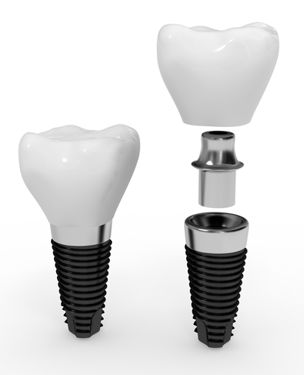
\includegraphics[width=0.4\textwidth]{grafiken/implant.png}
 	\caption{Single tooth replacement}
 	\label{fig:implant}
 \end{figure} 
 
 The crown of the tooth replacement is the part which imitates the visual qualities of the tooth. There are several material, which a crown can be made of or assembled from. The most popular crown material dominating the market is the Yttria-stabilized zirconia (YSZ), which has a cubic fluorite crystal structure and is going to be referred as zirconia in the frame of this thesis. However, zirconia in its pure form is a plain white material with high translucency. In case of single tooth replacement  the newle implanted crown would be absurdly white when compared to the neighboring teeth.Even when a full chin dental replacement is conducted, it is abnormal to have a full set of plain white teeth without any shading. This situation makes it a necessity to preprocess the crowns to match the neighboring teeth or another natural shade of choice in case of a fully monolithic replacement. Dentist are using a shade guide seen in the figure \ref{fig:shadeguide} for a side-by-side comparison to determine the color and the shade of the teeth. One can observe that there are 4 color groups A, B, C and D which are referred as orange-brown, yellow, grey-brown and red respectively \citep{vita}. Each of these colors have shades ranging from 1 to 4. Even though the shades are coded with the numbers from 1 to 4 with increments of 0.5 a total analogue shade acquisition is possible. The number 1 represents the shade with the least and 4 with the most saturated tone for each color.
 \newline
 \begin{figure}[h]
 	\centering
 	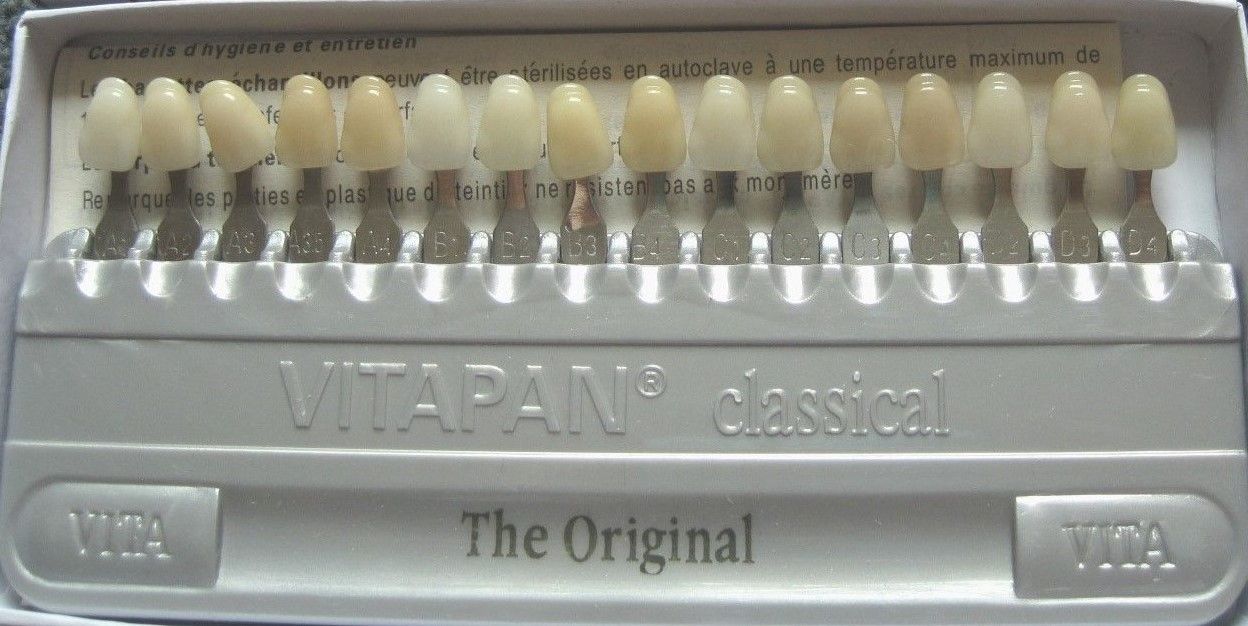
\includegraphics[width=0.9\textwidth]{grafiken/shadeguide.jpg}
 	\caption{Vitapan Shadeguide}
 	\label{fig:shadeguide}
 \end{figure}  
 


\chapter{State of the Research}
\label{sec:stand_forschung}
Addressing the shading process of the dental zirconia-based ceramics as a combined procedure of drop generation, dispersion of the ink within the porous material, generating the color below the surface of the printed area




\section{Drop Deployment}


\subsection{Piezoelectric}


\subsection{Electromagnetic}
\label{sec:freiheitsgrad_eines_getriebes}


\section{Ceramic coloring}
\label{sec:grundlagen_für_die_kinematischen_betrachtungen}


\chapter{State of the Technology}
\label{sec:stand_technik}
Even in the most contemporary dental laboratory of today's world, the coloring process is accomplished manually by a experienced dental technologist, who is following the guidelines prepared by the dental ink companies, which explain how a dental crown has to be colored sequentially using different colors on different areas of a single crown summarized in about 20 basic steps. The application of the ink on the dental crown with brush strokes takes about 5 minutes for each tooth depending on the manual measurements of the ink application process conducted by a dental technologist from Zirkonzahn for educational purposes.
On the left side you can see a cutout of a lab card. Dentists mark different areas of the crown with different colors from the guide for the technicians.
And on the right side are the tasks of a dental technician, which are mainly. Milling, Manually coloring using a brush, furnacing to burn the color to the Zirconia and lastly polishing for a natural look.
And the coloring part is the process, on which this thesis is focused.
\begin{figure}[h]
	\centering
	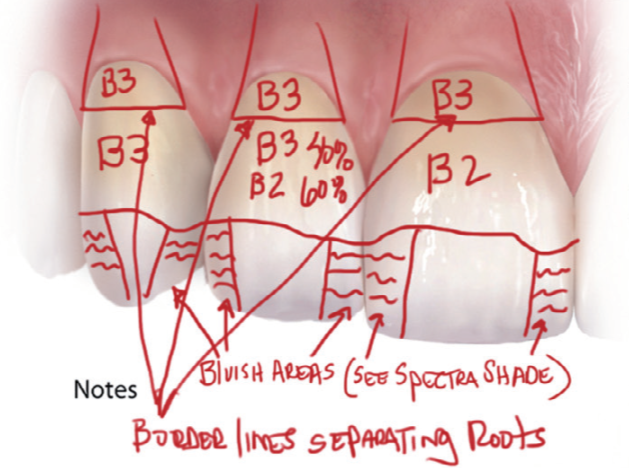
\includegraphics[width=0.5\textwidth]{grafiken/lab_card.png}
			\caption{Cutout of a lab card \citep{sharpling2014}}
	\label{fig:lab_card}
\end{figure}

\begin{figure}[h]
	\centering
	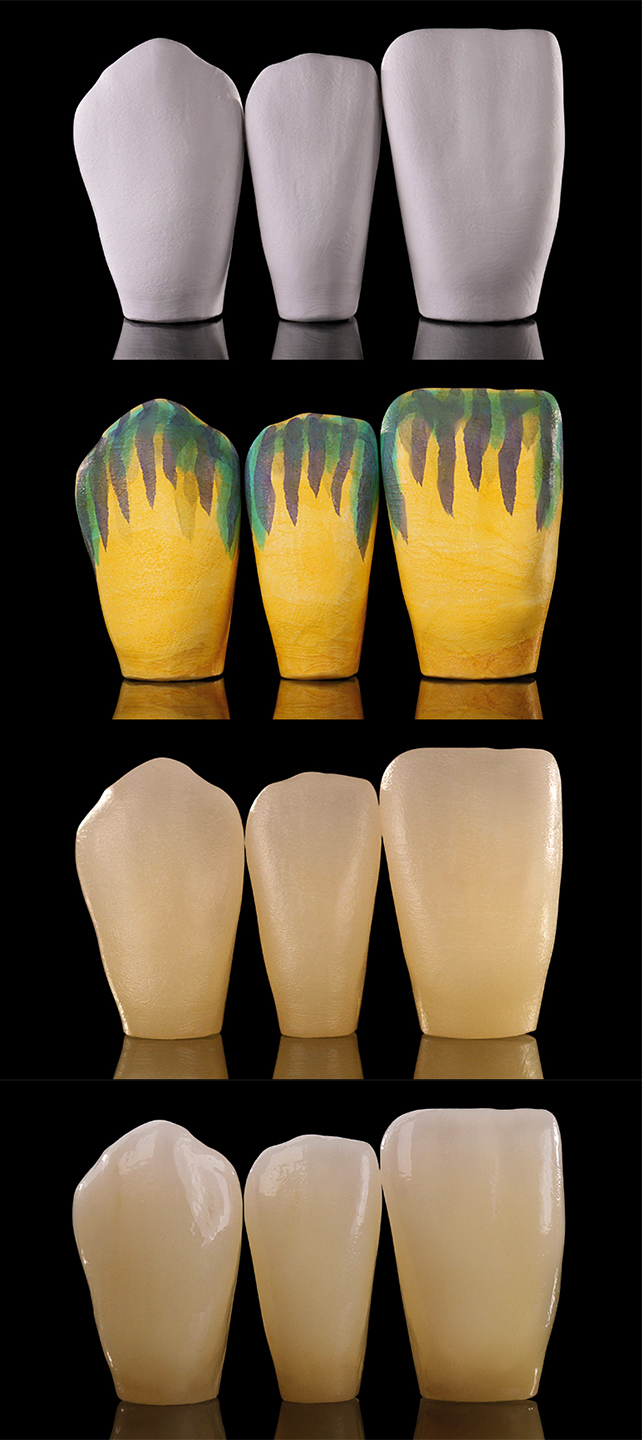
\includegraphics[height=0.6\textwidth]{grafiken/CrownProcesses.jpg}
	\caption{Making of dental implants \citep{zirkonzahn2018} }
	\label{fig:CrownProcesses}
\end{figure} 

\begin{figure}[h]
	\centering
	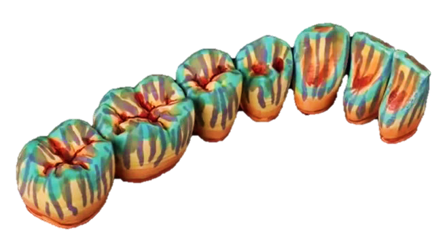
\includegraphics[width=0.6\textwidth]{grafiken/false_colored.png}
	\caption{False colored crowns after manual brushing \citep{zirkonzahn2018}}
	\label{fig:false_colored}
\end{figure}


\chapter{Review of the State of the Art and Technology}
\label{sec:kritik_stand_technik}
